\documentclass[a4paper, 12pt]{article}
%--------------------------------------
% Abstände
%--------------------------------------
\usepackage[left=30mm,right=20mm,top=25mm,headsep=15mm]{geometry}
\usepackage[onehalfspacing]{setspace}
%--------------------------------------
% encoding
%--------------------------------------
\usepackage[utf8]{inputenc}
\usepackage[T1]{fontenc}
%--------------------------------------
% Änderung Schriftart
% Quelle: http://www.math.tu-dresden.de/~rudl/latex/fonts.pdf
%--------------------------------------
\newcommand{\changefont}[3]{
\fontfamily{#1} \fontseries{#2} \fontshape{#3} \selectfont}
%--------------------------------------
% German-specific commands
%--------------------------------------
\usepackage[ngerman]{babel}
%--------------------------------------
% Hyphenation rules
%--------------------------------------
\usepackage{hyphenat}
\hyphenation{Sage Office Line GHS CLP gebinde-spezifische IDcmCallback FZPGHSDruckauftrag Untergruppen}
%--------------------------------------
% Hyperlinks
%--------------------------------------
\usepackage{url}
\usepackage{hyperref}
%--------------------------------------
% Grafiken
%--------------------------------------
\usepackage[rightcaption]{sidecap}
\usepackage{graphicx}
\usepackage{float}
\usepackage[skip=7pt]{caption}
\usepackage{here}
\graphicspath{{Images/}}
%--------------------------------------
% Enum
%--------------------------------------
\usepackage{enumitem}
%--------------------------------------
% Kopf-& Fußzeile
%--------------------------------------
\usepackage{color}
\definecolor{fzp}{rgb}{0.565,0.612,0.671}
\usepackage{fancyhdr}
\setlength{\headheight}{27pt}
\pagestyle{fancy}
\fancyhf{}
\renewcommand\headrule
{{\color{fzp}%
    \hrule height 3pt width \headwidth
    \vspace{1pt}%
	\hrule height 1pt width \headwidth
	\vspace{-4pt}
}}
%Fußzeile rechts
\fancyfoot[R]{\thepage}
%Fußzeile Plain
\fancypagestyle{plain}{ %
  \fancyhf{} % remove everything
  \renewcommand{\headrulewidth}{0pt} % remove lines as well
  \renewcommand{\footrulewidth}{0pt}
  \renewcommand{\headrule}{}
  \fancyfoot[R]{\thepage}
}
\setlength{\headsep}{20pt}
%--------------------------------------
% Fußnote 
%--------------------------------------
\usepackage[hang]{footmisc}
%--------------------------------------
% Quellcode 
%--------------------------------------
\usepackage{listings}
\definecolor{codegreen}{rgb}{0,0.6,0}
\definecolor{codeblue}{rgb}{0,0,1}
\definecolor{codepurple}{rgb}{0.58,0,0.82}
\definecolor{white}{rgb}{1,1,1}
\definecolor{black}{rgb}{0,0,0}
\lstset {
    breaklines=true,
    tabsize=3,
    showstringspaces=false
}
\lstdefinestyle{Common} {
    extendedchars=\true,
    language={[Visual]Basic},
    morekeywords={Using, As, New, Inherits, Class, Of},
    frame=single,
    %===========================================================
    framesep=3pt,%expand outward.
    framerule=0.4pt,%expand outward.
    xleftmargin=3.4pt,%make the frame fits in the text area. 
    xrightmargin=3.4pt,%make the frame fits in the text area.
    %=========================================================== 
    numbers=left,                    
    numbersep=-10pt,
    showspaces=false,                
    showstringspaces=false,
    showtabs=false,                  
    tabsize=1,
    captionpos=b
}
\lstdefinestyle{A} {
    style=Common,
    rulecolor=\color{black},
    backgroundcolor=\color{white},
    basicstyle=\scriptsize\color{black}\ttfamily,
    keywordstyle=\color{codeblue},
    identifierstyle=\color{black},
    stringstyle=\color{codepurple},
    commentstyle=\color{codegreen}
}
%--------------------------------------
% PDF 
%--------------------------------------
\usepackage{pdfpages}
%--------------------------------------
% Table 
%--------------------------------------
\usepackage{tabu}
%--------------------------------------
% Quellenverzeichnis 
%--------------------------------------
\usepackage{csquotes}
\usepackage[backend=biber,defernumbers,sorting=none,firstinits=true]{biblatex}
\addbibresource{biblo.bib}
%--------------------------------------
\begin{document}
%--------------------------------------
% großzügige Formatierungsweise
%--------------------------------------
\sloppy
%--------------------------------------
% Deckblatt
%--------------------------------------
\thispagestyle{empty}
\begin{center}
\Large{Berufsakademie Sachsen}
\end{center}
 
\begin{center}
\Large{Staatliche Studienakademie Leipzig}
\end{center}
\hspace{4cm}

\begin{center}
\textbf{\LARGE{Praxisarbeit}}
\end{center}

\begin{center}
\textbf{im Studiengang Informatik}
\end{center}
\hspace{4cm}

\begin{flushleft}
\begin{tabular}{l p{10pt} p{290pt}}
\\
\textbf{Thema:} & &  Entwicklung eines Erweiterungsmoduls für die Sage Office Line
zum Druck von Etiketten nach GHS / CLP Verordnung sowie eines Etikettendesigners\\
& & \\
& & \\
& & \\
\textbf{eingereicht von:} & & Sebastian Kloppe \\
& &                           Einertstraße 10\\
& &                           04315 Leipzig\\
& & \\
\textbf{Seminargruppe:} & & CS13-2 \\
\textbf{Matrikelnummer:} & & 5000349\\
& & \\
& & \\
\textbf{Betreuer:} & & B.Sc. Benjamin Teßmar\\
& &                    Funk, Zander \& Partner GmbH\\
& &                    Kreuzstraße 7\\
& &                    04103 Leipzig\\
& & \\
& & \\
& & \\
& & \\
& & \\
& & \\
& & \\
\textbf{eingereicht am:} & & 10. Juli 2015 in Leipzig\\
\end{tabular}
\end{flushleft}
%--------------------------------------
% Inhaltsverzeichnis
%--------------------------------------
\newpage
\pagenumbering{Roman}
\tableofcontents
%--------------------------------------
% Abbildungsverzeichnis
%--------------------------------------
\newpage
\listoffigures
\addcontentsline{toc}{section}{Abbildungsverzeichnis}
\renewcommand{\lstlistlistingname}{Quellcodeverzeichnis}
\lstlistoflistings
\addcontentsline{toc}{section}{Quellcodeverzeichnis}
%--------------------------------------
% Einleitung
%--------------------------------------
\newpage
\clearpage 
\pagenumbering{arabic}   

\section{Einleitung}
\label{sec:Einleitung}
Das Unternehmen, die Funk, Zander \& Partner GmbH, hat sich seit der Gründung im 
Jahr 1992 auf die elektronische Datenverarbeitung und Unternehmensberatung spezialisiert.
Das weitere Unternehmensangebot umfasst anwenderbezogene Schulungen und Programmierungsarbeiten.
Die Auseinandersetzung mit dem Thema "'Entwicklung  eines  Erweiterungsmoduls  für 
die  Sage Office Line zum Druck von Etiketten nach \emph{GHS/CLP}\footnote{\label{foot:ghs}
siehe \nameref{sec:Grundlagen} auf Seite \pageref{sec:Grundlagen}} Verordnung 
sowie eines Etikettendesigners"' ist im Rahmen einer Kundenanforderung entstanden.

\subsection{Motivation}
\label{subsec:Motivation}

Für Unternehmen der chemischen Industrie ist es notwendig, aufgrund neuer
gesetzlicher Bestimmungen zur Einstufung und Kennzeichnung von Chemikalien,
Etiketten nach \emph{GHS/CLP}\textsuperscript{\ref{foot:ghs}} Verordnung zu nutzen.
Aus diesem Grund ist es erforderlich für die Sage Office Line ein neues Modul zum Druck 
dieser Art von Etiketten zu entwickeln. Die Sage Office Line ist eine 
ERP\footnote{\label{foot:erp}
Enterprise-Resource-Planning: Effizente Planung / Steuerung von Unternehmensressourcen. 
\cite{ERP}} Softwarelösung der Firma Sage Software GmbH, welche eine 
Tochterfirma der britischen Sage Group ist. "'Sage gehört zu einem der größten 
Anbieter von Softwarelösungen und Services für den deutschen Mittelstand."' \cite{sage} 


\subsection{Zielsetzung}
\label{subsec:Zielsetzung}

Das Ziel ist die Schaffung eines Moduls zum Druck von Etiketten nach 
\emph{GHS/CLP}\textsuperscript{\ref{foot:ghs}} Verordnung zur Erweiterung des Funktionsumfangs 
des ERP - Systems der Sage Office Line. Diese Funktionsweise muss, aufgrund der gesetzlichen
Bestimmungen, bis zum 01. Juni 2015 umgesetzt und funktionsbereit sein\cite{ifag}. 
Des Weiteren war die Umsetzung des Eitkettendesigners bis zum 30. Juni 2015 angedacht.  
%--------------------------------------
% Grundlagen
%--------------------------------------
\newpage
\section{Grundlagen}
\label{sec:Grundlagen}
Die Abkürzung \emph{GHS/CLP} steht für \emph{Global Harmonized System of 
Classification and Labelling of Chemicals} (Global Harmonisiertes System zur 
Einstufung und Kennzeichnung von Chemikalien) der Vereinten Nationen. Ziel ist 
eine weltweite Angleichung von nationalen und regionalen Systemen. Dies ist 
eine verbindliche Verordnung und muss von allen Unternehmen der chemischen 
Industrie aus den Mitgliedsstaaten der Vereinten Nationen umgesetzt werden. 
Aus der Verordnung ergeben sich die Einführung von neuen Gefahrenpiktogrammen, 
Gefahrenklassen, höheren Einstufungen bekannter Stoffe und Gemische sowie 
Gefahren- und Sicherheitshinweise. \cite{ifag}

\subsection{Gefahrenpiktogramme}

Der Aufbau der Piktogramme ist ein auf der Spitze stehendes weißes Quadrat mit 
rotem Rand und schwarzem Symbol. Der größte Unterschied zu den alten Piktogrammen
ist die einheitliche Färbung aller Piktogramme. Auf der linken Seite der Abbildungen 
\ref{fig:umwgefahren} bis \ref{fig:gesgefahren} sind die alten Piktogramme zu sehen.
\begin{figure}[!ht]
    \centering
    
\includegraphics[height=80pt, width=\textwidth]{Piktogramm1.PNG}
    \caption[Piktogramme Teil 1]{\small{Piktogramme Teil 1. \cite{ifaa}}}
    \label{fig:pikto1}
\end{figure}

\noindent
Des Weiteren wurden folgende neue Symbole geschaffen:
\begin{figure}[!ht]
    \centering
    
\includegraphics[height=70pt, width=240pt]{Piktogramm2.PNG}
    \caption[Piktogramme Teil 2]{\small{Piktogramme Teil 2. \cite{ifaa}}}
    \label{fig:pikto2}
\end{figure}

\noindent
Unterhalb der Piktogramme müssen, je nach Notwendigkeit, die Signalwörter "'Gefahr"' für 
die gefährlichen Gefahrenkategorien und / oder "'Achtung"' für die weniger 
bedrohlichen Gefahrenkategorien verwendet werden. Ebenso wurden folgende 
Ersetzungsregeln für die Verwendung der Piktogramme definiert \cite{ifaa}:
\begin{itemize}[itemsep=0pt]
    \item Totenkopf ersetzt Ausrufezeichen (bisher: T ersetzt Xn, Xi)
    \item Ätzsymbol ersetzt Ausrufezeichen für Augen- oder Hautreizungen 
    (bisher: C ersetzt Xn, Xi)
    \item Bei Explosion ist Flamme und Brennender Kreis fakultativ, außer es gibt 
    Ausnahmen (bisher: E ersetzt F, O)
    \item Gesundheitsgefahr ersetzt Ausrufezeichen für Hautsensibilisierung oder 
    Haut- und Augenreizung
    \item Regel T ersetzt C - entfällt
\end{itemize}

\noindent
Mit den Abkürzungen \emph{T, Xn, Xi, E, F, O, C} sind die alten Bezeichnungen der Piktogramme 
gemeint, wobei \emph{T} für giftig / sehr giftig, \emph{Xn} und \emph{Xi} für 
gesundheitsschädlich / reizend, \emph{E} für explosionsgefährlich, \emph{F} und \emph{O}
für entzündlich / brandfördernd und \emph{C} für ätzend steht.

\subsection{Gefahrenklassen}

Die Einteilung der Gefahrenklassen besteht aus den folgenden drei Hauptgruppen mit Untergruppen:

\begin{table}[H]
\centering
\begin{tabu} to 1.0\textwidth { | X[l] | } \hline
  \textbf{Physikalische / Chemische Gefahren} \\ [0.5ex] \hline
    Explosive Stoffe/Gemische \& Erzeugnisse mit Explosivstoff \\ \hline
    Entzündbare Gase / Aerosole \\ \hline
    Oxidierende Gase / Flüssigkeiten / Feststoffe \\ \hline
    Gase unter Druck \\ \hline
    Entzündbare Flüssigkeiten / Feststoffe \\ \hline
    Selbstzersetzliche Stoffe und Gemische \\ \hline
    Pyrophore Flüssigkeiten / Feststoffe \\ \hline
    Selbsterhitzungsfähige Stoffe \& Gemische \\ \hline
    Stoffe \& Gemische, die in Berührung mit Wasser entzündbare Gase entwickeln \\ \hline
    Organische Peroxide \\ \hline
    Korrosiv gegenüber Metallen \\ \hline
  \textbf{Gesundheitsgefahren} \\ \hline 
    Akute Toxizität \\ \hline
    Ätz-/ Reizwirkung auf die Haut \\ \hline
    Schwere Augenschädigung / Augenreizung \\ \hline
    Sensibilisierung der Atemwege oder der Haut \\ \hline
    Keimzellmutagenität \\ \hline
    Karzinogenität \\ \hline
\end{tabu}
\end{table}

\begin{table}[H]
\centering
\begin{tabu} to 1.0\textwidth { | X[l] | } \hline
    Reproduktionstoxizität \\ \hline
    Spezifische Zielorgan-Toxizität (einmalige Exposition) \\ \hline
    Spezifische Zielorgan-Toxizität (wiederholte Exposition) \\ \hline
    Aspirationsgefahr \\ \hline
  \textbf{Umweltgefahren} \\ \hline
    gewässerschädigend \\ \hline
    die Ozonschicht schädigend (EU-spezifisch) \\ \hline
\end{tabu}
\end{table}

\subsection{Höhere Einstufung von Stoffen und Gemischen}

Des Weiteren ist eine meist höhere Einstufung bekannter Stoffe und Gemische 
vorzunehmen. Ein Beispiel hierfür ist, dass alle Gasflaschen, auch nicht-explosive 
Gase, zur neuen Gefahrenklasse „Gase unter Druck“ gehören und mit dem 
Gasflaschenpiktogramm gekennzeichnet werden müssen. Atemwegssensibilisierende 
Stoffe werden als gefährlich eingestuft und mit dem Symbol des menschlichen 
Umrisses ausgewiesen. \cite{dguv}

\subsection{Gefahren- und Sicherheitshinweise}

Ebenfalls wurden neue Gefahren- und Sicherheitshinweise geschaffen. Die neuen 
H-Sätze (Hazard Statements) sind wesentlich differenzierter als die alten R-Sätze 
(Risk Statements) und beschreiben Gefährdungen die von chemischen Stoffen 
ausgehen. Es müssen alle zutreffenden H-Sätze verwendet werden. Die neuen P-Sätze 
(Precautionary Statements) ersetzen die S-Sätze (Safety Statements) und geben 
Sicherheitshinweise zu Punkten Allgemeines, Prävention, Reaktion, Lagerung und 
Entsorgung. Auf dem Etikett können bis zu sechs P-Sätze verwendet werden (siehe 
Auflistung der H- und P- Sätze im Kapital \ref{sec:Anhang} - Anhang). \cite{dguv}

\subsection{Kennzeichnungsetikett nach GHS/CLP}

Das Etikett wird in der jeweiligen Amtssprache beschriftet, in dem der Stoff oder 
das Gemisch verkauft wird (mehrere Sprachen sind nicht ausgeschlossen). Das 
Etikett benötigt folgende Informationen \cite{dguv}:
\begin{itemize}[itemsep=0pt]
    \item Herstellerinformationen (Name, Adresse, Telefon) 
    \item Menge des Stoffes oder Gemisches
    \item Produktidentifikation
    \item Gefahrenpiktogramme (wenn vorhanden)
    \item Signalwort (wenn vorhanden)
    \item Gefahrenhinweise (wenn vorhanden)
    \item Sicherheitshinweise (wenn vorhanden)
    \item Ergänzende Informationen (wenn vorhanden)
\end{itemize}

\subsection{Gegenüberstellung alte / neue Einstufung \& Kennzeichnung}

Auf den Abbildungen \ref{fig:umwgefahren} bis \ref{fig:gesgefahren} sieht man die 
Änderungen der Einstufung \& Kennzeichnung nach \emph{GHS/CLP} Verordnung: 

\begin{figure}[H]
    \centering
    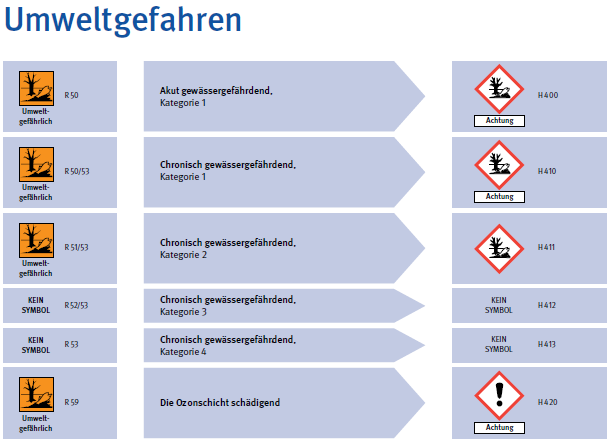
\includegraphics[height=300pt, width=\textwidth]{Gruppe3.PNG}
    \caption[Umweltgefahren]{\small{Umweltgefahren. \cite{bgw}}}
    \label{fig:umwgefahren}
\end{figure}

\begin{figure}[H]
    \centering
    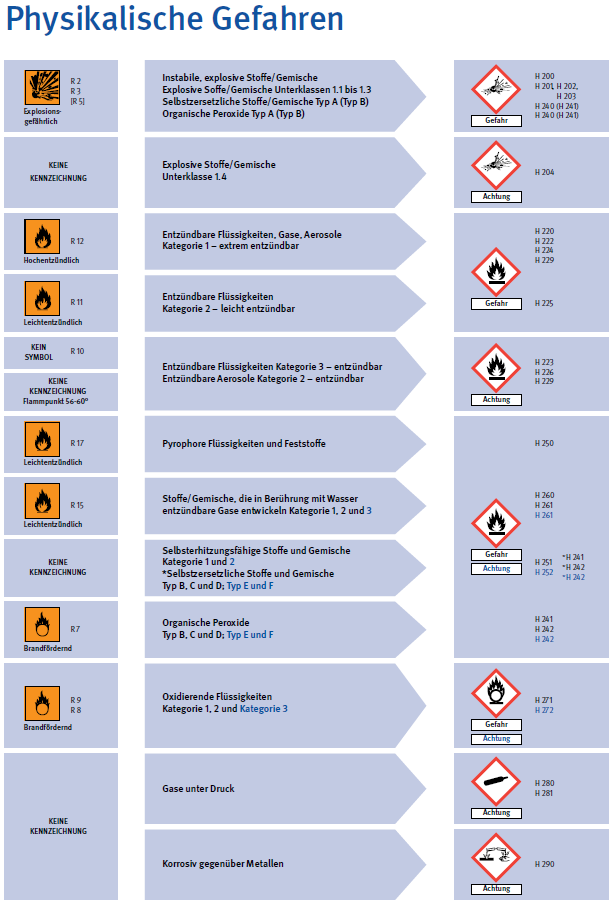
\includegraphics[height=590pt, width=\textwidth]{Gruppe1.PNG}
    \caption[Physikalische Gefahren]{\small{Physikalische Gefahren. \cite{bgw}}}
    \label{fig:phsgefahren}
\end{figure}

\begin{figure}[H]
    \centering
    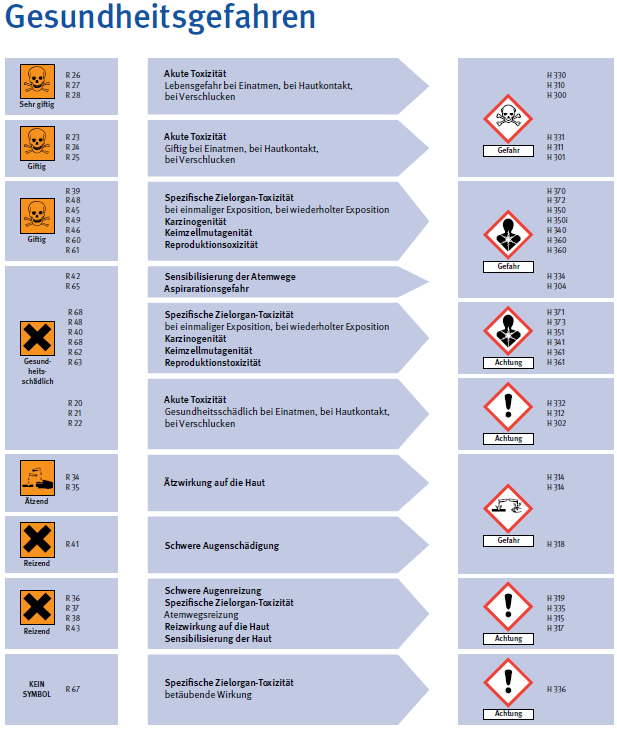
\includegraphics[height=560pt, width=\textwidth]{Gruppe2.PNG}
    \caption[Gesundheitsgefahren]{\small{Gesundheitsgefahren. \cite{bgw}}}
    \label{fig:gesgefahren}
\end{figure}

%--------------------------------------
% Konzeption
%--------------------------------------
\newpage
\section{Konzeption}
\label{sec:Konzeption}
\subsection{Anforderung}

Der Etikettendruckvorgang soll bei der Erstellung von Verkaufsbelegen, 
wie auch in der Lieferscheinauskunft ausgelöst werden. Als 
Anforderung ist die Schaffung eines Moduls zum Druck von Etiketten nach 
der \emph{GHS/CLP} Verordnung definiert. Das Etikett muss aussagekräftig
über den Hersteller (Name, Adresse, Telefon), der Menge des Stoffes oder 
Gemisches, der Produktidentifikation, der Gefahrenpiktogramme, der 
Signalwörter, der Gefahrenhinweise, der Sicherheitshinweise sowie über 
ergänzende Informationen sein. In Abbildung 
\ref{fig:musteretikett} ist ein solches Musteretikett sichtbar.

\begin{figure}[H]
    \centering
    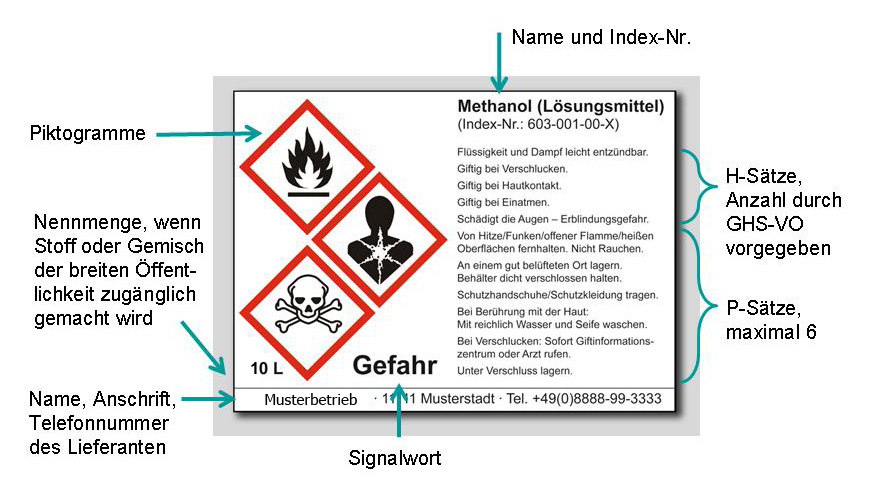
\includegraphics[height=200pt, width=320pt]{Beispieletikett.jpg}
    \caption[GHS Musteretikett]{\small{GHS Musteretikett. \cite{bgwetikett}}}
    \label{fig:musteretikett}
\end{figure}

\subsection{Ist-Zustand}

Gegenwärtig werden die Richtlinien nach der \emph{GHS/CLP} Verordnung für die 
Etiketten nicht von der Sage Office Line unterstützt. Aus diesem Grund werden 
bis zum Zeitpunkt der Moduleinführung die benötigten Etiketten, anhand einer PDF 
Vorlage, händisch von unserem Kunden erstellt. Die benötigten Daten hierfür 
kommen von einem Drittanbieter, welcher die Sicherheitsdatenblättern der 
jeweiligen Produkte erstellt. 

\noindent
Der derzeitige Ablauf der Etikettierung der Produkte erfolgt durch den 
Produktionsleiter. Dieser druckt anhand des Lieferscheins, 
direkt nach der Abfüllung des Produkts, das jeweilige händisch erstellte
Etikett mit der passenden Zweitsprache aus und klebt es auf die entsprechenden
Gebinde. Ein Gebinde ist eine Handelseinheit, welches Produkte gleicher Art bzw.
verschiedener Abfüllmengen zusammenfasst.\cite{gebinde} 
Bei der Abfüllung von Produkten in Säcken ist eine zusätzliche Etikettierung nicht notwendig, 
da diese bereits mit den benötigten \emph{GHS/CLP} Merkmalen bedruckt sind. \cite{fzp}

\begin{figure}[H]
    \centering
    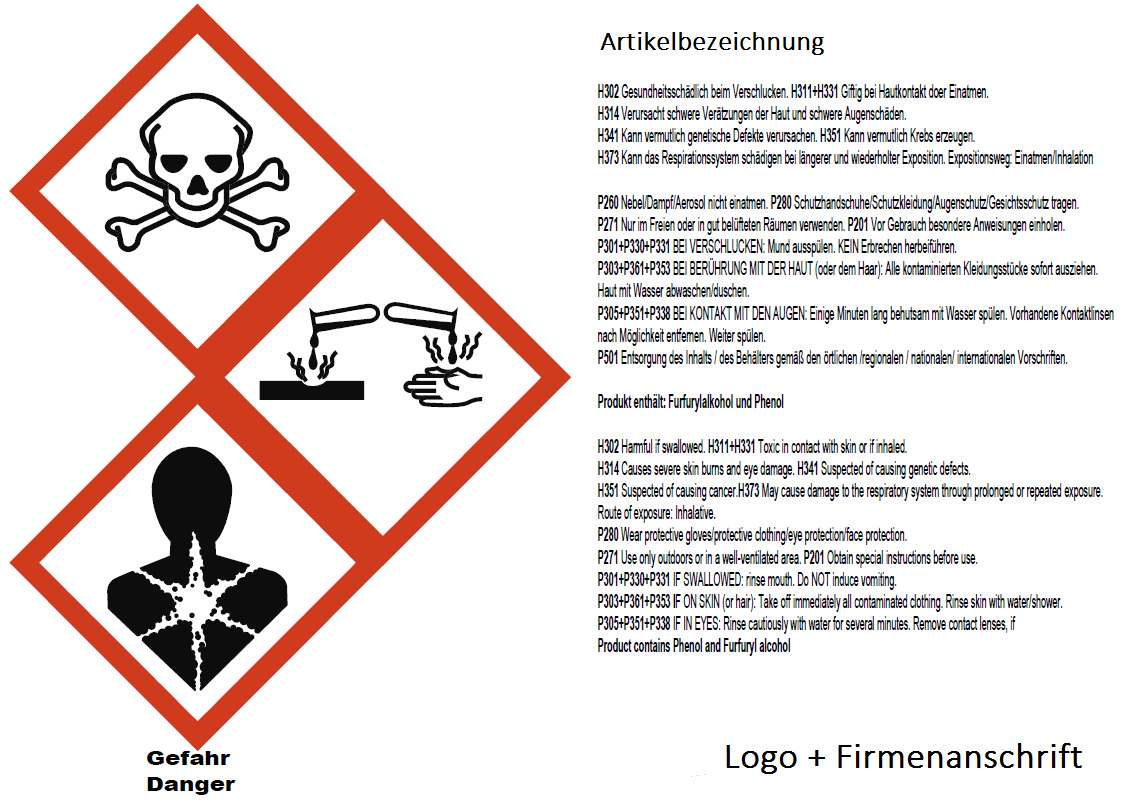
\includegraphics[height=280pt, width=400pt]{etikett_mod.png}
    \caption[händisch erstelltes Musteretikett]{\small{händisch erstelltes Musteretikett. \cite{fzp}}}
    \label{fig:hemusteretikett}
\end{figure}

\begin{figure}[H]
    \centering
    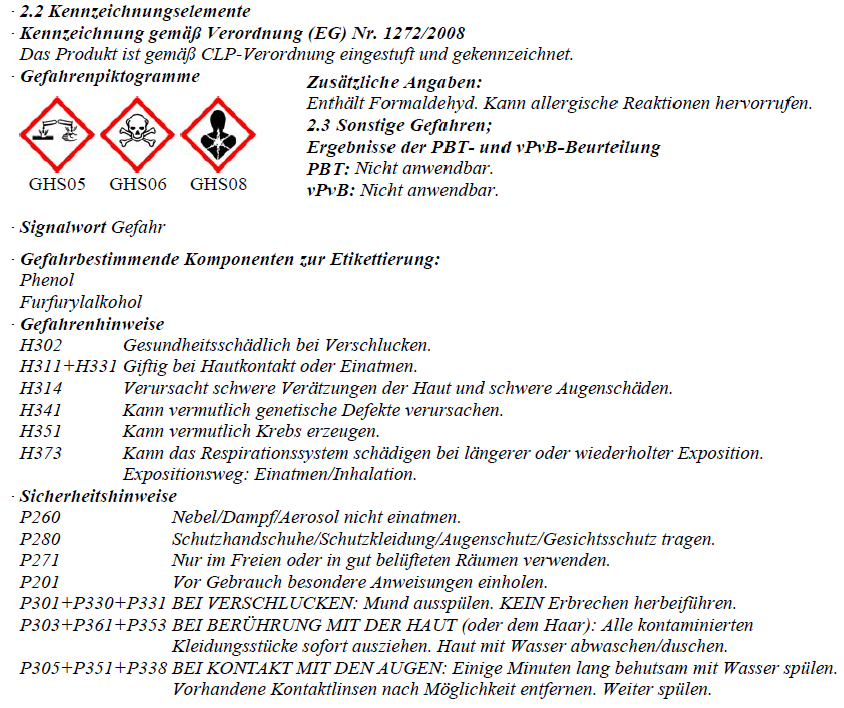
\includegraphics[height=285pt, width=330pt]{Sicherheitsdatenblatt.png}
    \caption[Muster Sicherheitsdatenblatt]{\small{Muster Sicherheitsdatenblatt. \cite{fzp}}}
    \label{fig:sicherheitsdatenblatt}
\end{figure}

\subsection{Ziele}
Das Hauptziel der Modulentwicklung ist die Abbildung der neuen gesetzlichen Voraussetzungen für 
Etiketten nach \emph{GHS/CLP} Verordnung in der Sage Office Line. Der Wechsel vom bestehenden,
manuellen Verfahren bis zur automatisierten Etikettenerzeugung ist ein weiteres Ziel. Daraus 
sollten zusätzliche Vorteile / Ziele resultieren, wie die Entlastung von Mitarbeitern, 
die Steigerung der Effizienz und die Reduzierung von Kosten.

\subsection{Planung}

Die Umsetzung des Projekts erfolgt in 2 Abschnitten. Im ersten Schritt 
ist es notwendig die Etiketten nach \emph{GHS/CLP} Verordnung 
zu erstellen und die Einbindung in die Sage Office Line zu realisieren. 
Der zweite Schritt umfasst die Programmierung des Etikettendesigners. Für die Entwicklung
des 1. Abschnitts war der Zeitraum von der 15. bis 19. Kalenderwoche sowie für den 2. Abschnitt 
der Zeitraum von der 20. bis 23. Kalenderwoche vorgesehen.

\subsubsection{Umstellung der Artikel}

Für eine bessere Zuordnung der Artikel zu den Etiketten wäre es vorteilhaft, 
gebindespezifische Artikel anzulegen. Dieser Schritt ist sinnvoll, da die 
Größe der Etiketten von der Füllmenge des Produktes abhängig ist. Jedoch ist 
dies ein größerer Eingriff in den aktuellen Unternehmensablauf und wird hier
nicht weiter berücksichtigt. Der Lösungsansatz um keine Prozesse ändern zu
müssen, ist der Aufruf einer Druckmaske nach dem Druck von Verkaufsbelgen 
oder Lieferscheinen. Mittels der Druckmaske lassen sich die Anzahl, wie auch 
die Größe der Etiketten nach \emph{GHS/CLP} Verordung für jeden Artikel
auswählen und drucken.

\begin{figure}[H]
    \centering
    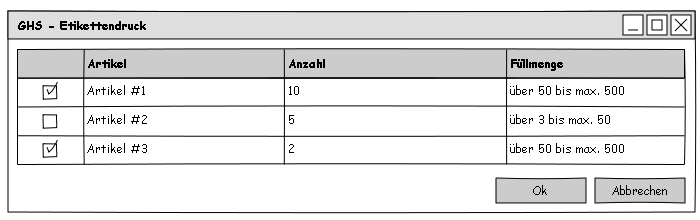
\includegraphics[height=130pt, width=\textwidth]{Druckmaske_2.png}
    \caption[Prototyp der Druckmaske]{\small{Prototyp der Druckmaske. \cite{fzp}}}
    \label{fig:prototypdruckmaske}
\end{figure}

\subsubsection{Erweiterung der Artikelstammdaten}
\label{subsubsec:erweiterungartikelstamm}

Zur Erstellung von Etiketten nach \emph{GHS/CLP} Verordnung ist es unabwendbar den 
Artikelstamm um die Eigenschaft „P-Sätze“ zu erweitern. Des Weiteren ist es 
erforderlich die Zweitsprache anhand der Adresse des Produktempfängers zu ermitteln. 
Die Auswahl der notwendigen Bestandteile der Etiketten erfolgt über fest 
definierte Auswahlfelder. Die Identifikationsnummern und Sprachpakete der 
offiziellen europäischen Amtssprachen stammen direkt von der Europäischen Union 
und werden mittels MS SQL\footnote{\label{foot:mssql}MS SQL: Die Abkürzung steht 
für Microsoft Structured Query Language und ist eine, von Microsoft entwickelte, 
Datenbanksprache für relationale Datenbanken "'zum Bearbeiten (Einfügen, Verändern, 
Löschen) und Abfragen von darauf basierenden Datenbeständen"'\cite{mssql}.}
– Skript bei Auslieferung des Moduls in die bestehende 
Datenbank integriert. Der Bezug der weiteren benötigten Sprachpakete für 
Arabisch (Ägyptisch), Chinesisch und Türkisch ist abschließend noch nicht 
geklärt. Es stehen diverse Online – Quellen von unterschiedlichen Anbietern zur Verfügung.
Die nachfolgende Abbildung zeigt die Erfassung der Arikelstammdaten vor der
geplanten Änderung.

\begin{figure}[H]
    \centering
    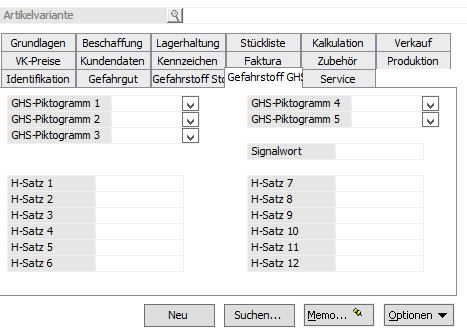
\includegraphics[height=230pt, width=320pt]{Artikelstamm.PNG}
    \caption[Arikelstammdatenerfassung]{\small{Arikelstammdatenerfassung. \cite{fzp}}}
    \label{fig:arikelstammdatenerfassung}
\end{figure}

\noindent
Die Abbildung \ref{fig:prototyparikelstammdatenerfassung} zeigt das geänderte Layout 
zur Erfassung der Artikelstammdaten anhand des Sicherheitsdatenblattes. Damit die 
Erfassung dynamisch gehalten werden kann, entfällt der Reiter \emph{Gefahrstoff GHS} 
im Artikelstamm (siehe Abbildung \ref{fig:arikelstammdatenerfassung}).

\begin{figure}[H]
    \centering
    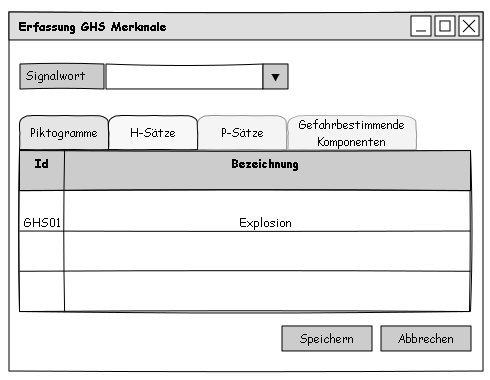
\includegraphics[height=170pt, width=330pt]{Stammdaten_3.png}
    \caption[Prototyp der Arikelstammdatenerfassung]
    {\small{Prototyp der Arikelstammdatenerfassung. \cite{fzp}}}
    \label{fig:prototyparikelstammdatenerfassung}
\end{figure}

\noindent
Die neue Erfassungsmaske kann über das Optionenmenü mittels dem Menüpunkt
\emph{GHS-Merkmale} ausgewählt werden. Weiterhin kann über den Menüpunkt
\emph{GHS-Etikettendesigner} der Etikettendesigner gestartet werden (siehe 
Abbildung \ref{fig:openerfassungsmaske1}).

\begin{figure}[H]
    \centering
    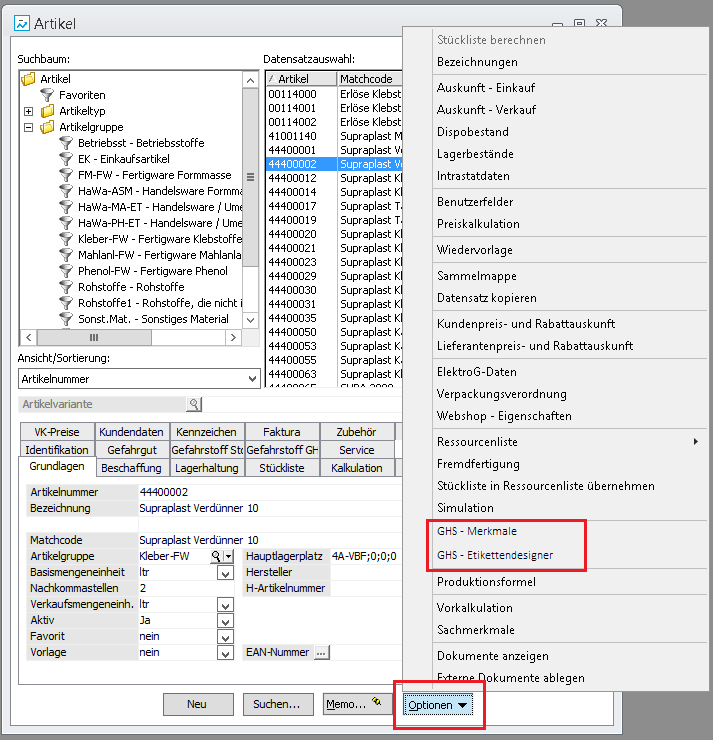
\includegraphics[height=360pt, width=430pt]{artikel_optionen_1.PNG}
    \caption[Öffnung Erfassungsmaske - Variante 1]
    {\small{Öffnung Erfassungsmaske - Variante 1. \cite{fzp}}}
    \label{fig:openerfassungsmaske1}
\end{figure}

\noindent
Außerdem können, wie in Abbildung \ref{fig:openerfassungsmaske2} zu sehen ist, 
über das Menü \emph{Extras | Schaltflächen} aus dem Optionsmenü 
Schaltflächen erzeugt werden, welche die Erfassungsmaske für die \emph{GHS/CLP} 
Merkmale sowie den Etikettendesigner direkt aufrufen können (GHS / Designer).

\begin{figure}[H]
    \centering
    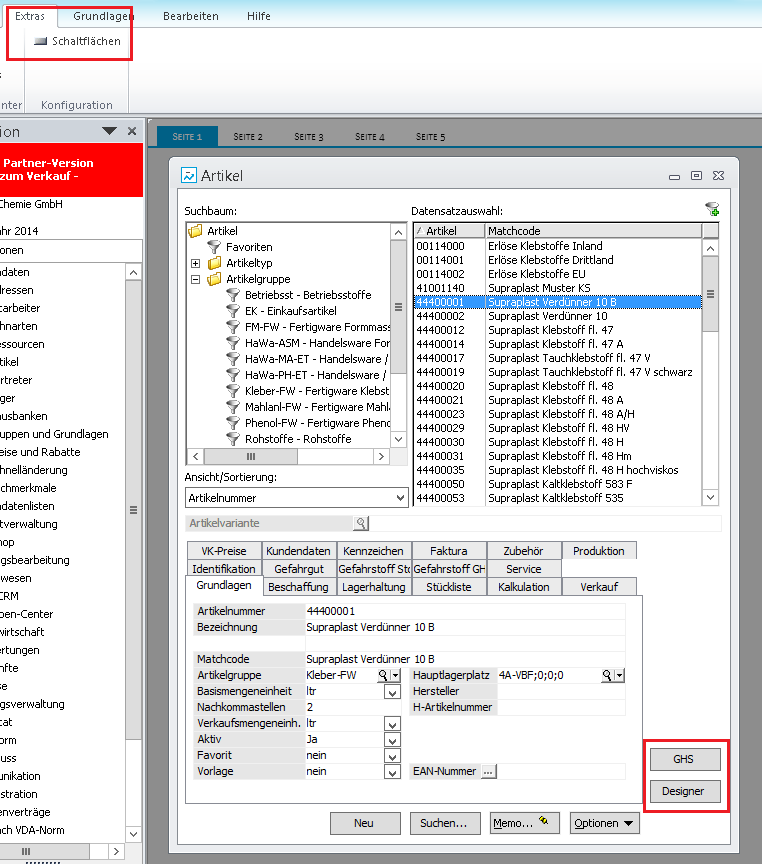
\includegraphics[height=410pt, width=430pt]{artikel_optionen_2.PNG}
    \caption[Öffnung Erfassungsmaske - Variante 2]
    {\small{Öffnung Erfassungsmaske - Variante 2. \cite{fzp}}}
    \label{fig:openerfassungsmaske2}
\end{figure}

\subsubsection{Erstellung der Etiketten}
\label{subsubsec:erstellungetiketten}
Zur Erstellung der Etiketten wird, anhand der gesetzlichen Vorgaben, eine selbst programmierte 
Vorlage verwendet. Hierbei ist zu beachten, dass die Größe der Etiketten sowie der Piktogramme 
an die Füllmenge des Produkts gekoppelt ist. Es müssen folgende Mindestabmessungen berücksichtigt 
werden:

\begin{table}[H]
\begin{tabular}{|l|l|l|}\hline
 \textbf{Füllmenge} & \textbf{Abmessung Etikett} & \textbf{Abmessung Piktogramm} \\
 \textbf{in l} & \textbf{in mm} & \textbf{in mm} \\ \hline
 bis 3 & wenn möglich min. 52 x 74 & min. 10 x 10, \\ & & wenn möglich 16 x 16 \\ \hline
 über 3 bis max. 50 & min. 74 x 105 & min. 23 x 23 \\ \hline
 über 50 bis max. 500 & min. 105 x 148 & min. 32 x 32 \\ \hline
 größer 500 & min 148 x 210 & min. 46 x 46 \\ \hline
\end{tabular}
\end{table}

\noindent
Die Etiketten sollen wie Folgt für die verschiedenen Piktogramm - Anzahlen aussehen:

\begin{figure}[H]
    \centering
    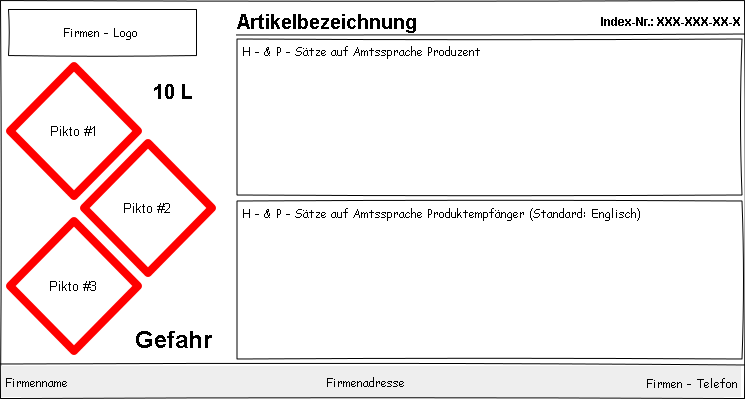
\includegraphics[height=170pt, width=340pt]{Musteretikett-3Pikto.png}
    \caption[Prototyp des Musteretiketts mit 3 Gefahrenpiktogramme]
    {\small{Prototyp des Musteretiketts mit 3 Gefahrenpiktogramme. \cite{fzp}}}
    \label{fig:prototypmusteretikett3p}
\end{figure}

\begin{figure}[H]
    \centering
    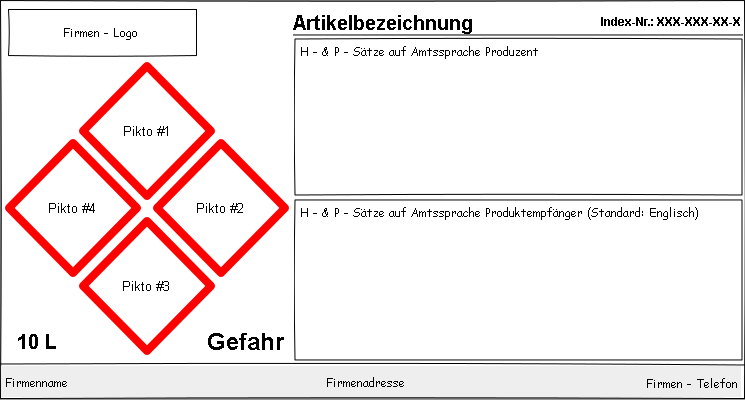
\includegraphics[height=170pt, width=340pt]{Musteretikett-4Pikto.png}
    \caption[Prototyp des Musteretiketts mit 4 Gefahrenpiktogramme]
    {\small{Prototyp des Musteretiketts mit 4 Gefahrenpiktogramme. \cite{fzp}}}
    \label{fig:prototypmusteretikett4p}
\end{figure}

\begin{figure}[H]
    \centering
    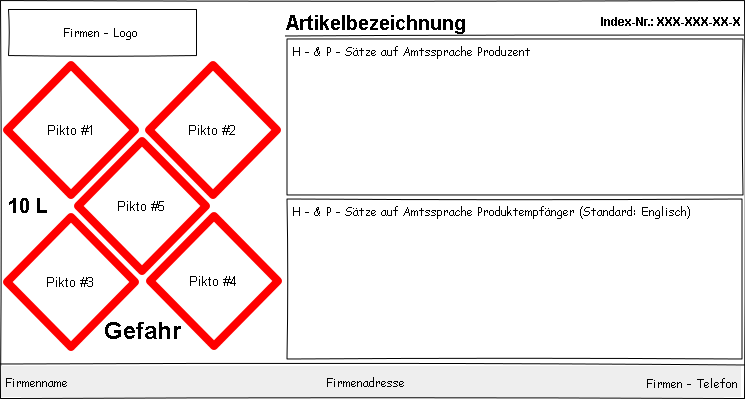
\includegraphics[height=170pt, width=340pt]{Musteretikett-5Pikto.png}
    \caption[Prototyp des Musteretiketts mit 5 Gefahrenpiktogramme]
    {\small{Prototyp des Musteretiketts mit 5 Gefahrenpiktogramme. \cite{fzp}}}
    \label{fig:prototypmusteretikett5p}
\end{figure}

\subsubsection{Erstellung des Etikettendesigner}
Mit dem Designer soll es möglich sein, Etiketten individuell gestalten zu können. 
Wichtig hierbei ist, dass bei selbsterstellten Etiketten die Prüfung der benötigten 
Etikettenbestandteile nach \emph{GHS/CLP} Verordnung vom Ersteller selbst 
durchgeführt werden muss. Der Designer soll ebenfalls, wie in Abbildung 
\ref{fig:openerfassungsmaske1} und \ref{fig:openerfassungsmaske2}
gezeigt, am Artikelstamm über das Optionsmenü aufgerufen werden können. 

\begin{figure}[H]
    \centering
    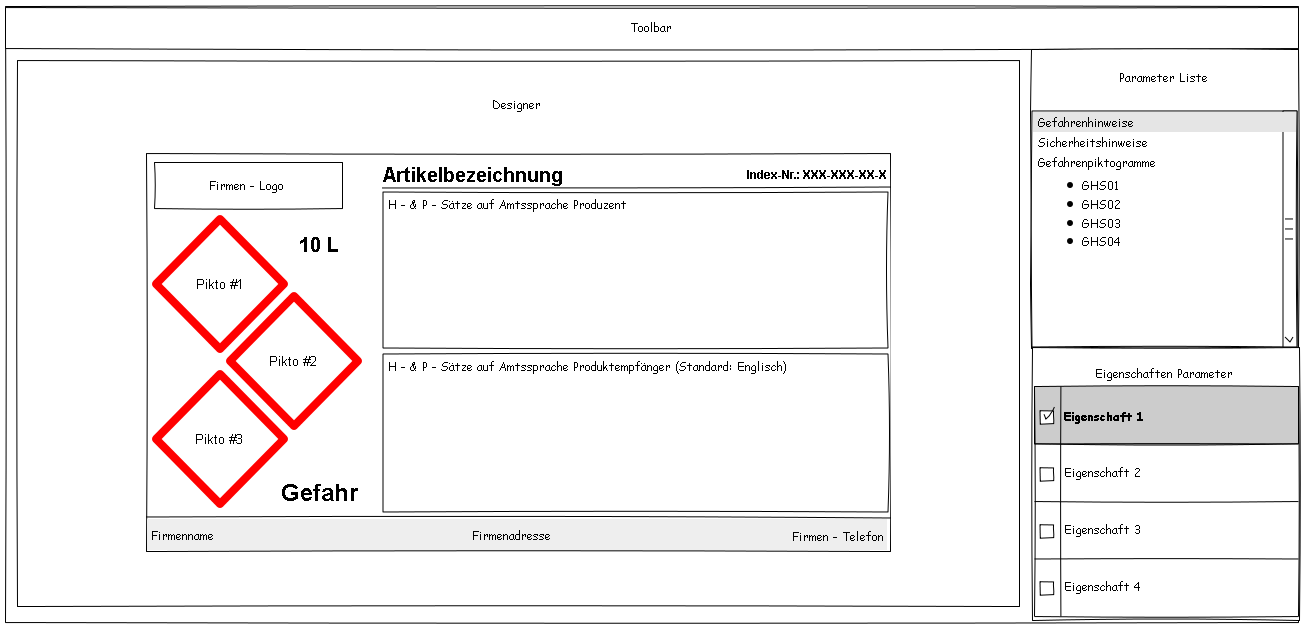
\includegraphics[height=240pt, width=\textwidth]{Etikettendesigner_1.png}
    \caption[Prototyp des Etikettendesigner]
    {\small{Prototyp des Etikettendesigner. \cite{fzp}}}
    \label{fig:prototypetikettendesigner}
\end{figure}
%--------------------------------------
% Umsetzung & Ergebnisse
%--------------------------------------
\newpage
\section{Umsetzung}
\label{sec:Umsetzung}
Die Entwicklung von Zusatzmodulen und Erweiterungen ist angesichts des modularen 
Aufbaukonzepts der Sage Office Line möglich. Die Einbindung von Erweiterungen wird 
mit einer eigenentwickelten Methode von Sage, namens DCM realisiert. Die Abkürzung
DCM steht für Dynamic Link Library\footnote{\label{foot:dll}Dynamic Link Library: 
Dynamische Programmbibliothek für Microsoft Betriebssysteme. (DLL) \cite{dll}} 
Common Method. Mit dieser Methode können Anpassung an der Sage Office Line auf Basis
des Microsoft .NET Frameworks\footnote{\label{foot:framework}Framework: Grundstruktur 
/ Rahmenwerk zur Bestimmung der Software-Architektur. Es besteht aus mehreren Klassen, 
die zusammenarbeiten und wieder verwendbare Entwürfe darstellen. \cite{framework}} 
vorgenommen werden. Mit Hilfe von DCM werden die Anpassungen mit der verwendeten 
Technologie der Sage Office Line auf Basis von Microsoft Access in Verbindung mit dem
Microsoft Component Object Model Frameworks (COM) verbunden.

\subsection{Projektstruktur}
Im ersten Schritt begann ich mit der Konstruktion der in Abbildung \ref{fig:paketdiagrammghs}
zu sehenden Projektstruktur. Zur Orientierung diente der vorher aufgestellte Umsetzungsplan.

\begin{figure}[H]
    \centering
    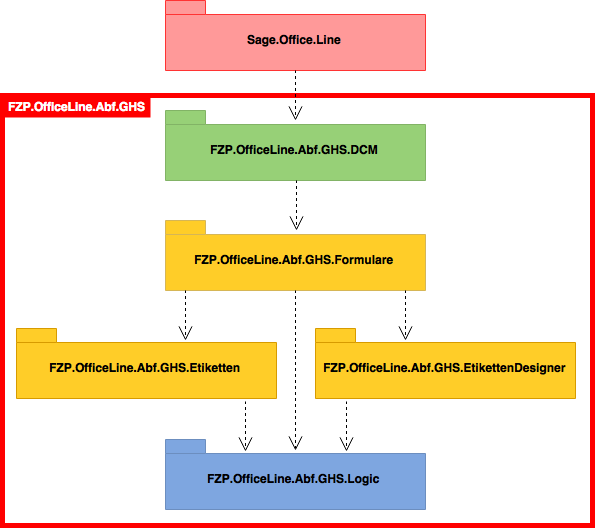
\includegraphics[height=240pt, width=300pt]{paketdiagramm_ghs_3.png}
    \caption[Paketdiagramm FZP.OfficeLine.Abf.GHS]
    {\small{Paketdiagramm FZP.OfficeLine.Abf.GHS}}
    \label{fig:paketdiagrammghs}
\end{figure}

\noindent
Das Projekt \emph{FZP.OfficeLine.Abf.GHS} unterteilt sich in 3 Bereiche. Das grün gefärbte
Paket stellt die Schnittstelle zwischen der Sage Office Line und dem Etikettendruckmodul 
dar. 

\begin{figure}[H]
    \centering
    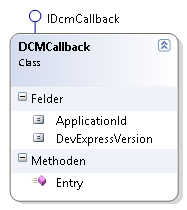
\includegraphics[height=100pt, width=90pt]{FZP_OfficeLine_Abf_GHS_DCM.png}
    \caption[Klassendiagramm FZP.OfficeLine.Abf.GHS.DCM]
    {\small{Klassendiagramm FZP.OfficeLine.Abf.GHS.DCM}}
    \label{fig:kddcm}
\end{figure}

\noindent
Die Schnittstelle, welche in Abbildung \ref{fig:kddcm} zu sehen ist, benötigt eine Klasse, 
welche das \emph{IDcmCallback} Interface von Sage implementiert. Dieses Interface stellt eine 
Methode namens \emph{Entry} zur Verfügung, welche ausimplementiert werden muss. Über diese 
Methode erhält man ein Kontext - Objekt, welches mit unterschiedlichen Daten (Kundennummer, 
Artikelnummer, Belegdaten, etc.) aus der Sage Office Line befüllt und in der Schnittstelle 
ausgelesen werden kann. 

\noindent
Die in der Abbildung \ref{fig:paketdiagrammghs} dargestellten gelb 
gefärbten Pakete repräsentiert die graphische Oberfläche des Moduls. Das Paket 
\emph{FZP.OfficeLine.Abf.GHS.Formulare} enthält die Klassen zur Erzeugung der Formulare. Die 
Formulare dienen einerseits zur Auswahl der Anzahl der zu druckenden Etiketten und deren 
Größe (\emph{frmGhsAuswahlEtiketten}). Auf der anderen Seite steht die Erfassung der Merkmale 
nach \emph{GHS/CLP} Verordnung für die einzelnen Artikel (\emph{frmGhsMerkmalErfassungsmaske}). 

\begin{figure}[H]
    \centering
    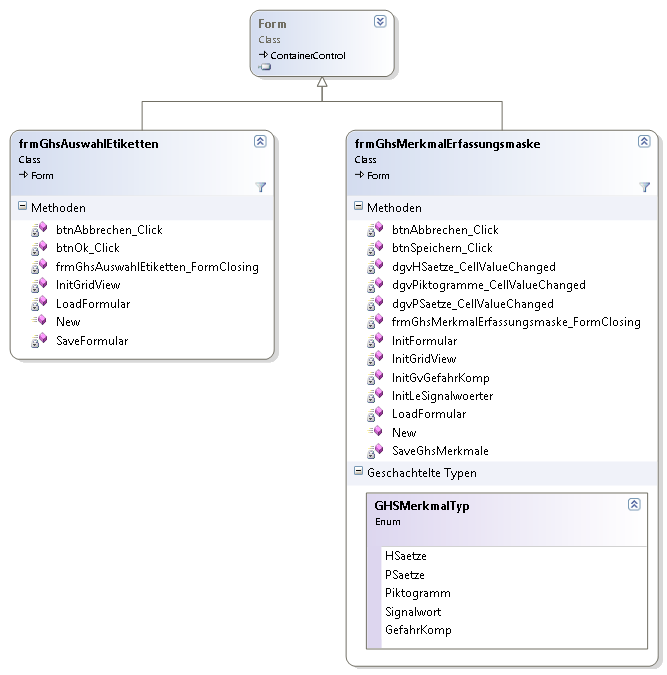
\includegraphics[height=290pt, width=290pt]{FZP_OfficeLine_Abf_GHS_Formulare_2.png}
    \caption[Klassendiagramm FZP.OfficeLine.Abf.GHS.Formulare]
    {\small{Klassendiagramm FZP.OfficeLine.Abf.GHS.Formulare}}
    \label{fig:kdformulare}
\end{figure}

\noindent
Das nächste Bestandteil ist das Paket \emph{FZP.OfficeLine.Abf.GHS.Etiketten}, welche die
notwendigen Klassen für die Erstellung der fest definierten Etiketten enthält. Für die
Etikettenerstellung kommt neben dem \emph{.NET} Framework, ein Framework der Firma 
Developer Express Inc. (DevExpress) zum Einsatz, welches die \emph{.NET} Winforms Steuerelemente 
im Funktionsumfang erweitert und zusätzlich die Handhabung erleichtert \cite{devexpress}. Zum Einen
enthält das Paket die Klasse \emph{GHSEtikettenAuswahl}, welche die Erstellung der Etiketten
anhand der übergebenen Füllmenge erzeugt, obendrein beinhaltet das Paket die konkreten Klassen 
für die einzelnen Etikettentypen. Außerdem sind die Gefahrenpiktogramme als Resourcen Dateien hinterlegt. 

\begin{figure}[H]
    \centering
    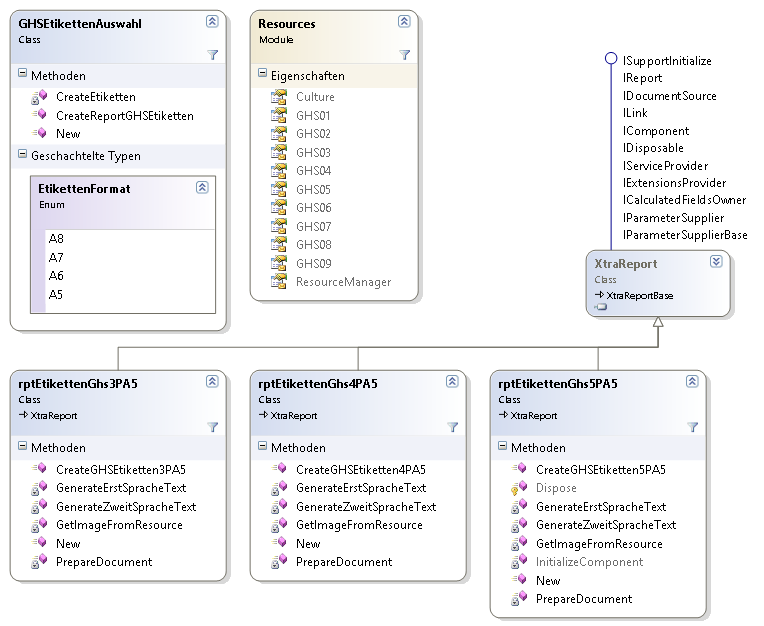
\includegraphics[height=300pt, width=\textwidth]{FZP_OfficeLine_Abf_GHS_Etiketten_2.png}
    \caption[Klassendiagramm Auszug FZP.OfficeLine.Abf.GHS.Etiketten]
    {\small{Klassendiagramm Auszug FZP.OfficeLine.Abf.GHS.Etiketten}}
    \label{fig:kdetiketten}
\end{figure}

\noindent
Die dritte Komponente ist das Paket \emph{FZP.OfficeLine.Abf.GHS.EtikettenDesigner}, 
welche die notwendigen Klassen für die Erstellung von selbst definierten Etiketten 
enthält. Auch hier wird neben dem \emph{.NET} Framework, dass Framework von \emph{DevExpress} 
verwendet. Leider wurde aufgrund zeitlicher und finanzieller Gründe der Etikettendesigner 
abschließend nicht von unserem Kunden beauftragt und ist somit nicht über die Planungsphase 
hinaus gekommen. Aus diesem Grund liegt nur eine grobe Klassenstruktur vor (siehe Abbildung 
\ref{fig:kdetikettendesigner}). 

\begin{figure}[H]
    \centering
    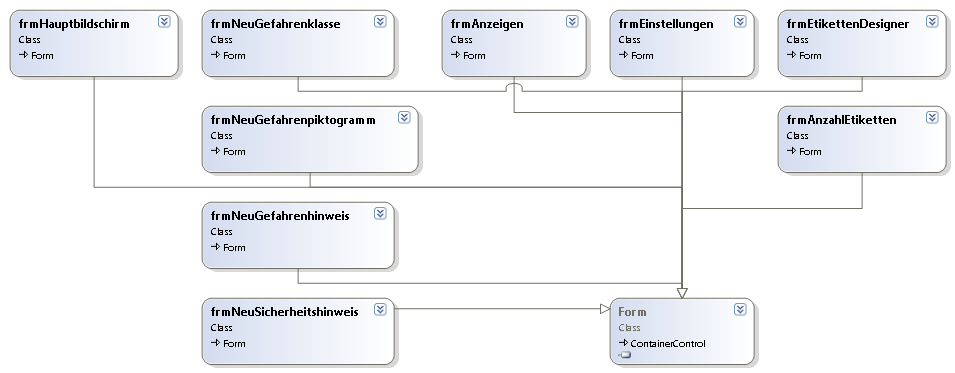
\includegraphics[height=250pt, 
    width=\textwidth]{FZP_OfficeLine_Abf_GHS_EtikettenDesigner_2.png}
    \caption[Klassendiagramm FZP.OfficeLine.Abf.GHS.EtikettenDesigner]
    {\small{Klassendiagramm FZP.OfficeLine.Abf.GHS.EtikettenDesigner}}
    \label{fig:kdetikettendesigner}
\end{figure}

\noindent
Das letzte Element des Moduls ist das blau gefärbte Paket \emph{FZP.OfficeLine.Abf.GHS.Logic}.
In diesem Paket befindet sich die Businesslogik des gesamten Etikettendruckmoduls. Das 
Hauptziel des Pakets ist die strikte Trennung der graphischen Oberfläche von der 
Businesslogik. Durch diese Trennung ist es möglich die graphische Oberfläche auszuwechseln ohne 
die Buisnesslogik ändern zu müssen. Das Paket beinhaltet Klassen zur Datenhaltung und Manipulation 
der Merkmale nach \emph{GHS/CLP} Verordnung. Die Klassen erben von der \emph{KeyedCollection} - Klasse, 
welche "'eine Basisklasse für eine Auflistung bereitstellt"' und mit Schlüssel - Wert Paaren 
arbeitet \cite{coll}. Die Speicherung der Daten erfolgt in der MS SQL Datenbank der Sage 
Office Line. Des Weiteren stellt das Paket zur Regelung der Datenbankverbindung und Ausführung 
von SQL - Abfragen Hilfsklassen zur Verfügung (GHSMerkmal, GHSMerkmalErweiterung, MandantHelper). 
Daneben steht eine Klasse zur Größenänderung von Bildern, Umwandlung von Bilder in den Datentyp 
\emph{Byte Arrays} und umgekehrt zur Verfügung (ImageHelper). Weiterhin existiert eine Klasse zur
Aufbereitung der Daten aus der Datenbank zur Verwendung in der graphischen Oberfläche (GHSMerkmalHelper) 
(siehe Abbildung \ref{fig:kdlogik}).

\begin{figure}[H]
    \centering
    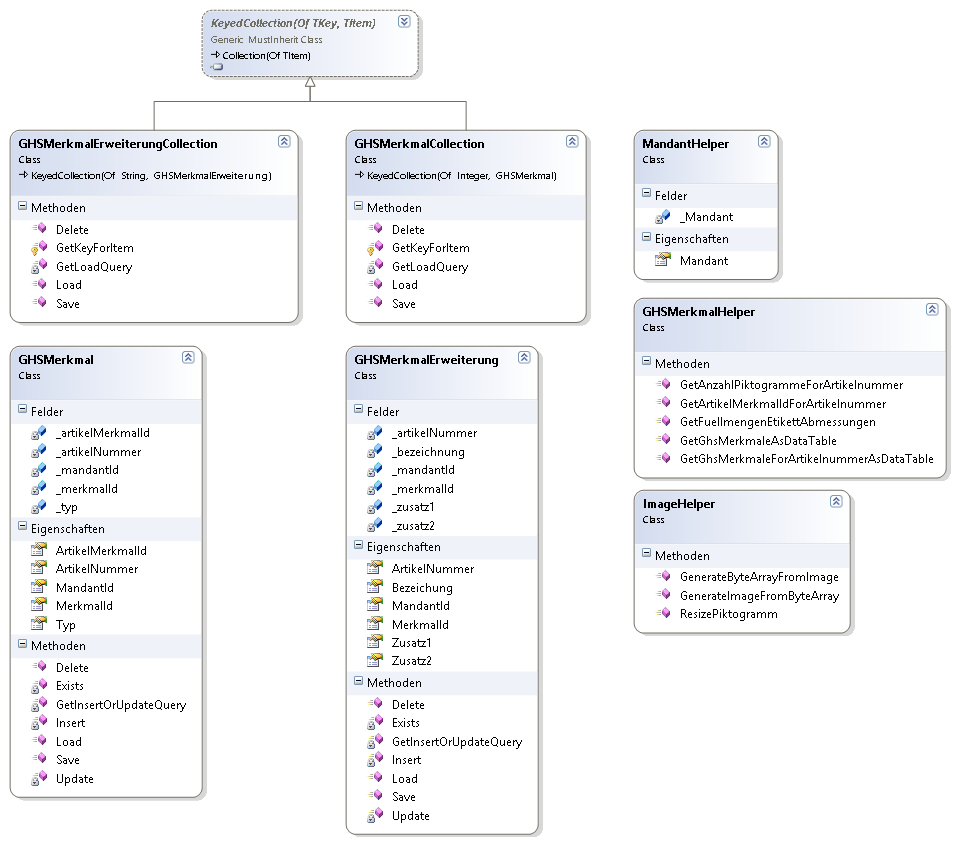
\includegraphics[height=450pt, width=\textwidth]{FZP_OfficeLine_Abf_GHS_Logic_2.png}
    \caption[Klassendiagramm FZP.OfficeLine.Abf.GHS.Logic]
    {\small{Klassendiagramm FZP.OfficeLine.Abf.GHS.Logic}}
    \label{fig:kdlogik}
\end{figure}

\subsection{Funktionsweise}

Im nachfolgenden Abschnitt ist die Funktionsweise des Moduls anhand von Quellcodeauszügen
erklärt. Das Etikettendruckmodul wird, wie in Abschnitt \ref{subsubsec:erweiterungartikelstamm}
bereits erläutert wurde, an mehreren Stellen aufgerufen. Dabei kann der Anwender
in der Sage Office Line den Menüpunkt "'GHS Merkmale"' in den Artikelstammdaten auswählen
(Case Zweig 201). Nach der Speicherung von Verkaufsbelegen wird das Ereignis 
"'FZPGHSDruckauftrag"' ausgelöst (Case Zweig 200). Das Modul arbeitet den folgenden Quellcode ab:
\newline
\newline
\newline
\begin{lstlisting}[style=A, caption=Aufruf Formulare aus Sage Office Line (COM),
label={code:addin}]
    Select Case nMode
        '# Aufruf Formular Druckauftrag
        Case 200
            Set oBagDCM = New ParameterBag
            Set oBagDCM.oItem("Beleg") = goStack.oBag.oItem("Beleg")
            Call goMandant.bExecuteDCMCustomizing("FZPGHSDruckauftrag", oBagDCM)
            
        '# Aufruf Formular Erfassung GHS Merkmale
        Case 201
            Set oBagDCM = New ParameterBag
            oBagDCM.sItem("Artikelnummer") = gsParameter(sArgs, "Artikelnummer", "")
            Call goMandant.bExecuteDCMCustomizing( _
            "FZPGhsErfassungMerkmaleArtikelstamm", oBagDCM)
    End Select
\end{lstlisting}

\noindent
Wie zu sehen ist wird in beiden Case Zweigen ein Objekt von Typ \emph{ParameterBag} erzeugt. 
Dieses Objekt dient zur Übergabe und Haltung von Daten aus der Sage Office Line in unser 
Modul. Der Einstiegspunkt in das Etikettendruckmodul ist zu sehen in der Zeile 6 und 
Zeile 12 des Quellcodes. Die Methode \emph{bExecuteDCMCustomizing} benötigt 2 Parameter. 
Der erste Parameter muss eine eindeutige Zeichenketten sein, welche zur Identifikation in
unserem Modul genutzt wird, um festzustellen welche Funktion ausgewählt wurde (siehe Listing
\ref{code:addin}: Zeile 6 und 12 und Listing \ref{code:dcmcallback}: Zeile 2 und 10). Als 
zweiter Parameter wird das erzeugte \emph{ParameterBag} Objekt übergeben. Im 
Quellcodeauszug Nr. \ref{code:dcmcallback} sieht man die Auswertung der übergebenen
Zeichenkette in der \emph{Select Case Anweisung}, außerdem das Auslesen und die Verarbeitung des
Kontext - Objekts (siehe Zeile 4 - 6 und Zeile 12 - 14).

\begin{lstlisting}[style=A, caption=Verarbeitung Aufruf Formulare aus Sage Office Line (.NET),
label={code:dcmcallback}]
    Select Case context.Listname
        Case "FZPGHSDruckauftrag"
            '# Aufruf Formular zum Druck der Etiketten
            Dim dcmBeleg As Sagede.OfficeLine.Wawi.BelegEngine.DcmContextBeleg = _
            CType(context, Sagede.OfficeLine.Wawi.BelegEngine.DcmContextBeleg)
            Dim beleg As Sagede.OfficeLine.Wawi.BelegEngine.Beleg = dcmBeleg.Beleg
            Using druckAuftrag As New frmGhsAuswahlEtiketten(mandant, beleg)
                druckAuftrag.ShowDialog()
            End Using
        Case "FZPGhsErfassungMerkmaleArtikelstamm"
            '# Aufruf Formular zu Erfassung der GHS Merkmale
            Dim engine As DcmContextEngine = CType(context, DcmContextEngine)
            Dim artikelNummer As String = engine.ParameterBag.StringValues( _ 
            "Artikelnummer")
            Using merkmalErfassungsmaske As New frmGhsMerkmalErfassungsmaske(Mandant, _
            artikelNummer)
                merkmalErfassungsmaske.ShowDialog()
            End Using
    End Select
\end{lstlisting}

\noindent
Nach der Verarbeitung des Kontext-Objekts zur Verwendung der übergebenen Daten aus der Sage
Office Line folgt die Initialisierung der Formulare. Zum Einen für die Aufnahme der Merkmale nach 
\emph{GHS/CLP} Verordnung für den übergebenen Artikel (Abbildung \ref{fig:eperfassungsmaske})
oder zum Anderen für den Aufruf der Druckmaske (Abbildung \ref{fig:epdruckmaske}) (siehe Listing
\ref{code:dcmcallback} - Quellcodezeilen 7 - 9 plus 15 - 18).

\begin{figure}[H]
    \centering
    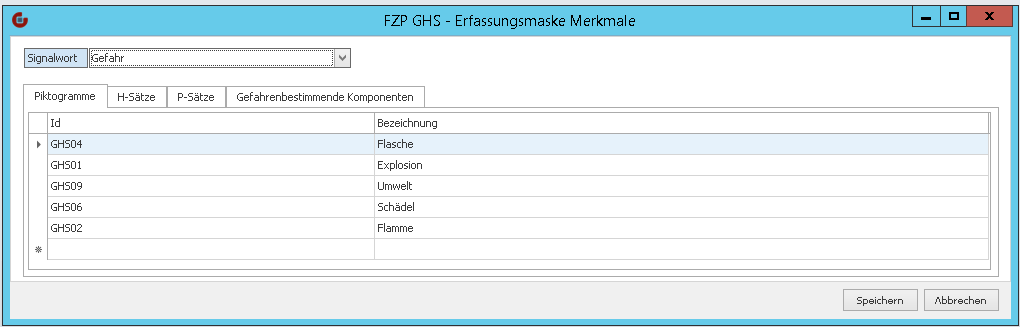
\includegraphics[height=160pt, width=\textwidth]{Erfassung_endprodukt_2.png}
    \caption[Endprodukt der Arikelstammdatenerfassung]
    {\small{Endprodukt der Arikelstammdatenerfassung}}
    \label{fig:eperfassungsmaske}
\end{figure}

\noindent
Die erste Möglichkeit ist die Erfassung der benötigten Merkmale nach \emph{GHS/CLP} Verordnung für 
jeden einzelnen Artikel (siehe Abbildung \ref{fig:eperfassungsmaske}). Durch Betätigung der Schaltfläche
zum Speichern werden die Informationen in die MS SQL Datenbank geschrieben (siehe Listing \ref{code:speichern}).
\newline
\begin{lstlisting}[style=A, caption=Auszug Speicherroutine GHS/CLP Merkmale (.NET),
label={code:speichern}]
    Public Class frmGhsMerkmalErfassungsmaske
        ...
        '# Aufruf Methode zur Speicherung GHS Merkmale im Formular 
        '# mittels Speichern Button
        '# ----------------------------------------------------------------
        '# Die eingegebenen Daten werden aus der GridView in eine DataTable 
        '# geschrieben. Anschlieszend werden alle Zeilen der DataTable 
        '# durchgegangen und die Daten in Objekte geschrieben und der 
        '# Collection hinzugefuegt und abschlieszend gespeichert.  
        Private Function SaveGhsMerkmale() As Boolean
            dgvHSaetze.UpdateCurrentRow()
            ...
            Dim hSaetze As DataTable = CType(dgcHSaetze.DataSource, DataTable)
            ...
            Dim ghsMerkmale As New GHSMerkmalCollection
            Dim ghsMerkmal As GHSMerkmal
            Dim artikelMerkmalId As Integer
            ...
            '# H-Saetze
            For Each row As DataRow In hSaetze.Rows
                ghsMerkmal = New GHSMerkmal
    
                If FZPCInt(row("ArtikelMerkmalId")) = 0 Then
                    artikelMerkmalId = _mandant.GetTan("FZPGHSArtikelMerkmal")
                Else
                    artikelMerkmalId = FZPCInt(row("ArtikelMerkmalId"))
                End If
                ghsMerkmal.ArtikelMerkmalId = artikelMerkmalId
                ghsMerkmal.MandantId = _mandant.Id
                ghsMerkmal.ArtikelNummer = _artikelNummer
                ghsMerkmal.Typ = GHSMerkmalTyp.HSaetze
                ghsMerkmal.MerkmalId = FZPCStr(row("MerkmalId"))
    
                ghsMerkmale.Add(ghsMerkmal)
            Next
            ...
            If ghsMerkmale.Save() Then
                Return True
            End If
        End Function
        ...
    End Class

    Public Class GHSMerkmalCollection
        Inherits System.Collections.ObjectModel.KeyedCollection(Of Integer, GHSMerkmal)
        ...
        '# Aufruf Speicheranweisung aller GHS Merkmal Objekte innerhalb der Collection
        Public Function Save() As Boolean
            For Each item As GHSMerkmal In Me
                item.Save()
            Next
        End Function
        ...
    End Class
    
    Public Class GHSMerkmal
        ...
        '# Ausfuehrung der Speicheranweisung fuer jedes GHS Merkmal
        '# ----------------------------------------------------------------
        '# Zuerst wird der SQL-Query mittels StringBuilder erstellt. Die @-Parameter 
        '# dienen als Platzhalter die durch die "sqlCommand.AppendInParameter()" 
        '# Anweisung durch die Daten aus dem GHS Merkmale Objekt ersetzt werden. 
        '# Mittels der Anweisung "sqlCommand.ExecuteNonQuery()" wird der SQL-Query 
        '# auf der Datenbank ausgefuehrt.
        Private Sub Save()
            Try
                Dim query As New System.Text.StringBuilder
                
                query.AppendLine("INSERT INTO FZPGHSArtikelMerkmal")
                query.AppendLine("(")
                query.AppendLine("  ArtikelMerkmalId,")
                query.AppendLine("  Mandant,")
                query.AppendLine("  Typ,")
                query.AppendLine("  MerkmalId,")
                query.AppendLine("  Artikelnummer")
                query.AppendLine(")")
                query.AppendLine("VALUES")
                query.AppendLine("(")
                query.AppendLine(" @ArtikelMerkmalId,")
                query.AppendLine(" @Mandant,")
                query.AppendLine(" @Typ,")
                query.AppendLine(" @MerkmalId,")
                query.AppendLine(" @Artikelnummer")
                query.AppendLine(")")
                
                Dim sqlCommand As IGenericCommand = 
                MandantHelper.Mandant.MainDevice.GenericConnection.CreateCommand( _
                GenericCommandType.SqlS
                tring, query.ToString, True)
                sqlCommand.AppendInParameter("ArtikelMerkmalId", GetType(Integer), _
                _artikelMerkmalId)
                sqlCommand.AppendInParameter("Mandant", GetType(Short), _mandantId)
                sqlCommand.AppendInParameter("Typ", GetType(Integer), _typ)
                sqlCommand.AppendInParameter("MerkmalId", GetType(String), _merkmalId)
                sqlCommand.AppendInParameter("Artikelnummer", GetType(String), _
                _artikelNummer)
    
                sqlCommand.ExecuteNonQuery()
            Catch ex As Exception
                Throw New Exception("Speichern der GHS-Merkmal mit ID " & _
                _artikelMerkmalId & " fehlgeschlagen." & _
                Environment.NewLine & ex.Message)
            End Try
        End Sub
        ...
    End Class
\end{lstlisting}

\begin{figure}[H]
    \centering
    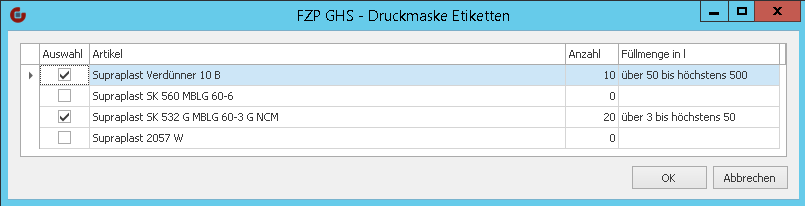
\includegraphics[height=140pt, width=\textwidth]{druckmaske_endprodukt_2.png}
    \caption[Endprodukt der Druckmaske]
    {\small{Endprodukt der Druckmaske}}
    \label{fig:epdruckmaske}
\end{figure}

\noindent
Die zweite Möglichkeit ist der Aufruf der Druckmaske nach dem Speichern eines Verkaufsbeleges. 
Diese zeigt alle Artikel des jeweiligen Verkaufsbeleges an. Hier kann entschieden werden, für 
welche Artikel Etiketten erstellt werden sollen. Zudem kann die Anzahl und die Größe des
Etiketts angegeben werden (siehe Abbildung \ref{fig:epdruckmaske}). Die Größe des Etiketts wird 
anhand der Füllmenge bestimmt, wie im Abschnitt \ref{subsubsec:erstellungetiketten} der Konzeption beschrieben. 
Mit Betätigung der OK Schaltfläche wird die Etikettenerstellung ausgelöst. Das Endprodukt der 
Erstellung ist in Abbildung \ref{fig:epetikett} zu sehen. Die Erstellung der Etiketten wird auszugsweise 
im Listing \ref{code:etiketten} beschrieben.

\begin{figure}[H]
    \centering
    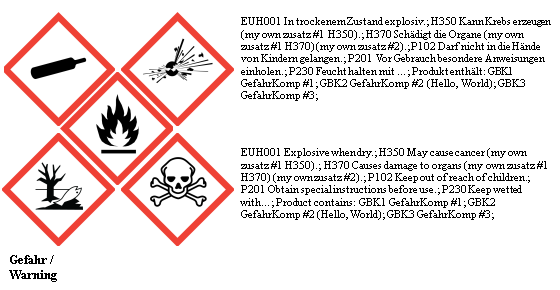
\includegraphics[height=210pt, width=\textwidth]{musteretikett_endprodukt.PNG}
    \caption[Endprodukt der Etiketten]
    {\small{Endprodukt der Etiketten (ohne kundenspezifischer Angaben)}}
    \label{fig:epetikett}
\end{figure}

\begin{lstlisting}[style=A, caption=Auszug Routine Etikettenerstellung (.NET),
label={code:etiketten}]
    Public Class frmGhsAuswahlEtiketten
        ...
        '# Aufruf Methode zur Etikettenerstellung im Formular mittels OK Button
        '# ----------------------------------------------------------------
        '# Die eingegebenen Daten werden aus der GridView in eine DataTable 
        '# uebergeben und eine neue Instanz des Objekts zur Auswahl der Etiketten
        '# mittels der uebergebenen Daten erzeugt. Anschlieszend wird die Methode 
        '# "CreateReportGHSEtiketten()" aufgerufen die die Etiketten erstellt. 
        Private Function SaveFormular() As Boolean
            ...
            Dim druckAuftraege As DataTable = dataRows.CopyToDataTable
            Dim ghsEtikettenAuswahl As New GHSEtikettenAuswahl(druckAuftraege)
            ghsEtikettenAuswahl.CreateReportGHSEtiketten() 
            ...
        End Function
        ...
    End Class
    
    Public Class GHSEtikettenAuswahl
        ...
        '# Die uebergebene DataTable wird zeilenweise durchgegangen und
        '# anhand der Fuellmenge wird entschieden welches Etikettenformat
        '# genommen werden soll. Anschlieszend wird Methode "CreateEtiketten()"
        '# ausgefuehrt die die Etiketten anhand der Anzahl der Piktogramme erstellt.
        Public Function CreateReportGHSEtiketten() As Boolean
            For Each row As DataRow In _dtDruckAuftraege.Rows
                Dim artikelNummer As String = FZPCStr(row.Item("Artikelnummer"))
                Dim artikelZielland As String = FZPCStr(row.Item("Zielland"))
                Dim auswahlEtikettenFormat As Integer = FZPCInt(row.Item("Fuellmenge"))
                Dim anzahlPiktogramme As Integer = _
                GHSMerkmalHelper.GetAnzahlPiktogrammeForArtikelnummer(artikelNummer)
                ...
                Select Case auswahlEtikettenFormat
                    ...
                    Case EtikettenFormat.A5
                        CreateEtiketten(anzahlPiktogramme, artikelNummer, _
                        artikelZielland, artikelBezeichnung, anzahl)
                        Return True
                End Select
            Next
        End Function
    
        '# Erstellung Etiketten anhand der Piktogrammanzahl mittels der Methode
        '# "CreateGHSEtiketten3PA5()" der Klasse "rptEtikettenGhs3PA5".
        Private Sub CreateEtiketten(ByVal anzahlPiktogramme As Integer, _
          ByVal artikelnummer As String, ByVal artikelZielland As String, _
          ByVal artikelBezeichnung As String, ByVal anzahl As Integer)
            Select Case anzahlPiktogramme
                ...
                Case 3
                    Using report3p As New rptEtikettenGhs3PA5(artikelnummer, _
                      artikelZielland, artikelBezeichnung, anzahl)
                        report3p.CreateGHSEtiketten3PA5()
                    End Using
                ...
            End Select
        End Sub
        ...
    End Class

    Public Class rptEtikettenGhs3PA5
        ...
        '# Zuerst werden die GHS Merkmal Daten anhand der uebergebenen
        '# Artikelnummer von der Datenbank geladen. Danach wird die Zweitsprache
        '# fuer das Etikett bestimmt. Anschlieszend werden die Etiketten mittels
        '# der Methode "PrepareEtikett()" erstellt. Im letzten Schritt werden 
        '# die erzeugten Etiketten dem Anwender mit der Anweisung
        '# "mainReport.ShowPreviewDialog()" zum drucken angezeigt.
        Public Sub CreateGHSEtiketten3PA5()
            Dim ghsMerkmale As DataTable = 
            GHSMerkmalHelper.GetGhsMerkmaleForArtikelnummerAsDataTable(_artikelNummer)
            Dim ghsMerkmaleZweitsprache As DataTable
    
            If "DE".Equals(_artikelZielland) Then
                ghsMerkmaleZweitsprache = 
                GHSMerkmalHelper.GetGhsMerkmaleForArtikelnummerAsDataTable( _ 
                _artikelNummer, False, 0, Nothing, "EN")
            Else
                ghsMerkmaleZweitsprache = 
                GHSMerkmalHelper.GetGhsMerkmaleForArtikelnummerAsDataTable( _ 
                _artikelNummer, False, 0, Nothing, _artikelZielland)
            End If
    
            Dim mainReport As New XtraReport
            mainReport.PaperKind = Printing.PaperKind.A4
    
            For i As Integer = 1 To _anzahl
                If Me.PrepareEtikett(ghsMerkmale, ghsMerkmaleZweitsprache) Then
                    Me.CreateDocument()
                    mainReport.Pages.Add(Me.Pages.Item(0))
                End If
            Next
    
            mainReport.ShowPreviewDialog()
        End Sub
        
        '# In dieser Methode werden alle GHS Merkmale mit dem Etikett
        '# verknuepft, z.B. mit den Anweisungen "Me.pbPiktogramm1.Image" 
        '# oder "Me.lblSignalwort.Text".
        Private Function PrepareEtikett(ByVal ghsMerkmale As DataTable, _
          ByVal ghsMerkmaleZweitsprache As DataTable) As Boolean
            If ghsMerkmale Is Nothing Then Return False
            ...
            Dim piktogrammRows As List(Of DataRow) = (From row As DataRow _ 
            In ghsMerkmale.AsEnumerable Where row.Field(Of String) _
            ("MerkmalId").StartsWith("GHS")).ToList
            
            For Each row As DataRow In piktogrammRows
                If piktogrammRows.IndexOf(row) = 0 Then
                    Me.pbPiktogramm1.Image = 
                    ImageHelper.ResizePiktogramm(GetImageFromResource( _
                    FZPCStr(row.Item("MerkmalId"))), 115, 115)
                End If
                ...
            Next
    
            Dim sbSW As New System.Text.StringBuilder
            Dim signalwortRows As List(Of DataRow) = (From row As DataRow In _
            ghsMerkmale.AsEnumerable Where row.Field(Of String) _ 
            ("MerkmalId").StartsWith("SW")).ToList
            
            For Each row As DataRow In signalwortRows
                sbSW.Append(FZPCStr(row.Item("Bezeichnung")))
            Next
    
            sbSW.Append(" / ")
    
            Dim signalwortZSRows As List(Of DataRow) = (From row As DataRow In _
            ghsMerkmaleZweitsprache.AsEnumerable Where row.Field(Of String) _
            ("MerkmalId").StartsWith("SW")).ToList
            
            For Each row As DataRow In signalwortZSRows
                sbSW.Append(FZPCStr(row.Item("Bezeichnung")))
            Next
            Me.lblSignalwort.Text = sbSW.ToString
            ...
            Return True
        End Function
        ...
    End Class
\end{lstlisting}

%--------------------------------------
% Zusammenfassung
%--------------------------------------
\newpage
\section{Zusammenfassung}
\label{sec:Zusammenfassung}
Der Ausgangspunkt für die Auseinandersetzung mit dem Thema "'Entwicklung  eines  
Erweiterungsmoduls für die  Sage Office Line zum Druck von Etiketten nach \emph{GHS/CLP} 
Verordnung sowie eines Etikettendesigners"' war ein Kundenauftrag. Das Ziel des Kundenauftrags 
ist die Einführung einer automatisierten Lösung zur Umsetzung der neuen gesetzlichen 
Verpflichtung für die chemische Industrie. Daraus folgt die Etikettierung der Waren mittels der 
Schaffung eines Zusatzmoduls für die Sage Office Line.
\newline 
\newline
\noindent
Die Anbindung einer Erweiterung ist hinsichtlich des modularen Aufbaus der Sage Office Line 
möglich. Die verwendete Technologie in der Softwareentwicklung basiert auf dem Microsoft .NET 
Framework in Verbindung mit Microsoft Access und dem Microsoft COM Framework. Die Verwaltung der 
Daten wurde mit einem Microsoft SQL Server realisiert. 
\newline
\newline
\noindent
Das Ergebnis ist eine voll integrierte Erweiterung für die Sage Office Line, welche die 
gesetzlichen Voraussetzung zur Etikettierung erfüllt. Ein weiteres 
Resultat der Entwicklung ist die wiederverwendbare Logik zur Erstellung von Etiketten anhand
von Daten aus einer MS SQL Datenbank. Als zusätzlicher Einsatzort wäre die Erstellung von 
Adressetiketten für den Versand möglich. An dieser Stelle wäre die Schaffung eines Zusatzmoduls im Bereich 
Adressverwaltung / Kundenstammdaten denkbar. Des Weiteren soll perspektivisch die Entwicklung 
des ursprünglich geplanten Etikettendesigner als internes Projekt durchgeführt werden. Der 
Etikettendesigner soll sowohl innerhalb der Sage Office Line, wie auch ohne vorhandener Sage 
Office Line als eigenständige Softwarelösung nutzbar sein.


%--------------------------------------
% Anhang
%--------------------------------------
\newpage
\section{Anhang}
\label{sec:Anhang}
\begin{figure}[H]
    \centering
    
\includegraphics[angle=90, height=610pt, 
    width=\textwidth]{hpSaetze1.PNG}
    \caption*{Auflistung der H- und P- Sätze Teil 1 \cite{baua}}
    \label{fig:hpsaetze1}
\end{figure}

\begin{figure}[H]
    \centering
    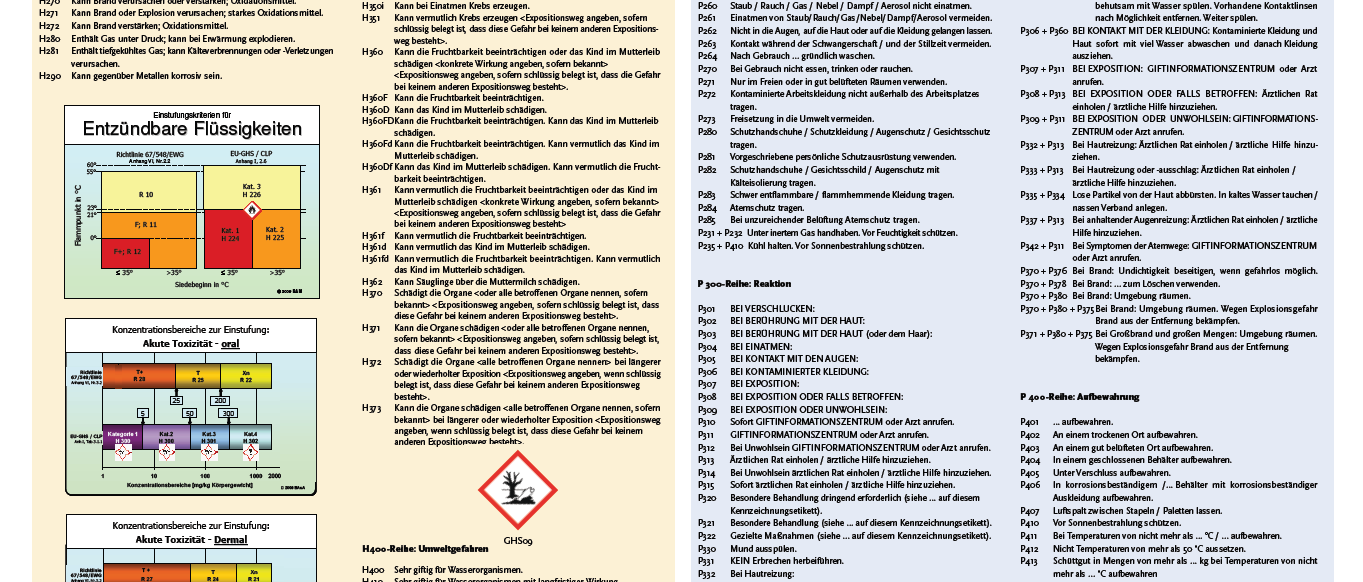
\includegraphics[angle=90, height=640pt, 
    width=\textwidth]{hpSaetze22.PNG}
    \caption*{Auflistung der H- und P- Sätze Teil 2 \cite{baua}}
    \label{fig:hpsaetze2}
\end{figure}

\begin{figure}[H]
    \centering
    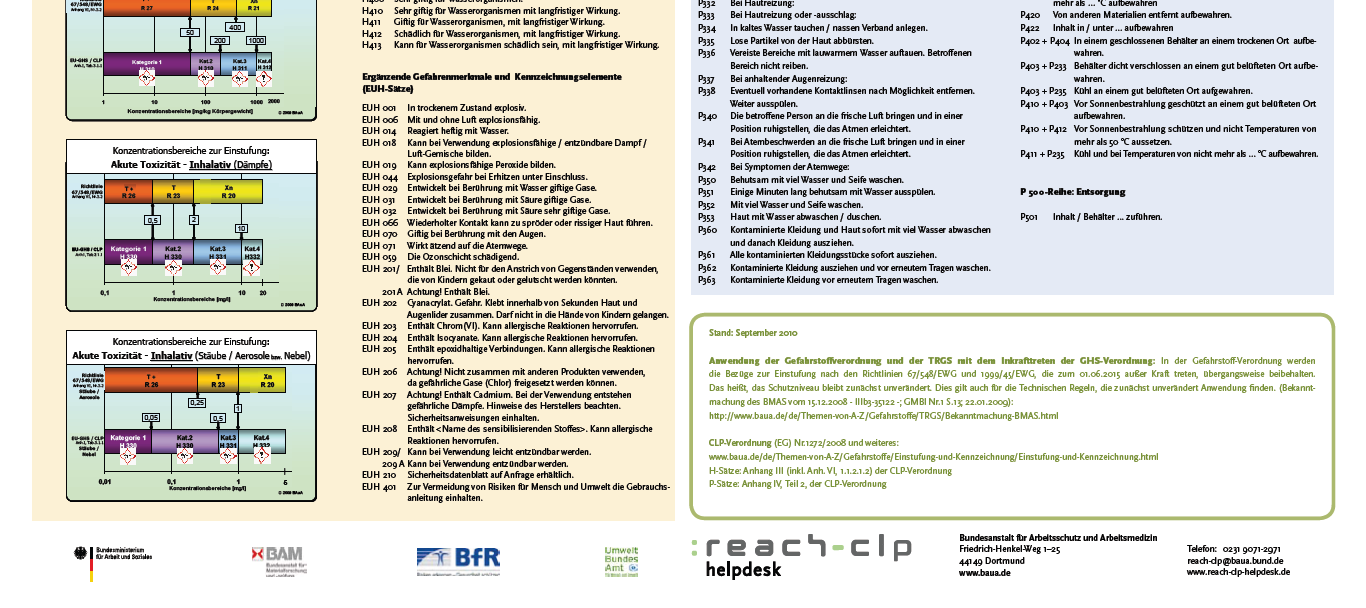
\includegraphics[angle=90, height=640pt, 
    width=\textwidth]{hpSaetze32.PNG}
    \caption*{Auflistung der H- und P- Sätze Teil 3 \cite{baua}}
    \label{fig:hpsaetze3}
\end{figure}

%--------------------------------------
% Quellenverzeichnis
%--------------------------------------
\newpage
\section{Quellenverzeichnis}
\printbibliography[title={ }]
%--------------------------------------
% Selbststänigkeitserklärung
%--------------------------------------
\newpage
\section*{Selbstständigkeitserklärung}
\normalsize{Ich versichere, dass ich die vorliegende Arbeit ohne fremde Hilfe 
selbstständig verfasst und nur die angegebenen Quellen und Hilfsmittel benutzt habe. 
Wörtlich oder dem Sinn nach aus anderen Werken entnommene Stellen sind unter Angabe der 
Quellen kenntlich gemacht. Die Arbeit wurde bisher in gleicher oder ähnlicher Form weder 
veröffentlicht, noch einer anderen Prüfungsbehörde vorgelegt.
\newline
\newline
\newline
\newline
Leipzig, den \today}
\end{document}